Effective written communication requires both sound content and clear style. Keep the layout of your thesis neat and pay attention to your writing style.

\section{Text}

Do not worry about the layout of the text, this template takes care of it already. Brief basics of writing style:
\begin{itemize}
\item Always think of your reader when you are writing and proceed logically from general to specific.
\item Highlight your key points, for example, by discussing them in a separate \verbcommand{section} or \verbcommand{subsection}, or presenting them in a table or figure. Use italics (\verbcommand{emph}) for emphasis, but don’t overdo it. 
\item Avoid long sentences and complicated statements. A full stop is the best way to end a sentence. 
\item Use active verbs to make a dynamic impression but avoid the first person pronoun I, except in your preface. 
\item Avoid jargon and wordiness. Use established terminology and neutral language.
\item The minimum length of sections and subsections is two paragraphs, and you need to consider the balance of chapters. Paragraphs must always consist of more than one sentence. 
\item Do not use more than three levels of numbered headings, such as 4.4.2. This is covered already by the template.
\item Do not use too many abbreviations. Use capital and small letters consistently.
\end{itemize}

\section{Figures}

You must refer to all the figures in the body text. The reference should preferably appear on the same page as the actual figure or before it. Figures and tables must be numbered consistently and primarily placed at the top of the page, but you are free to decide where they fit best. \LaTeX{} takes care of the numbering, if you specify a unique \verbcommand{label} right after the \verbcommand{caption} of a figure (or a table). Cross-referencing is done by inserting this identifier as the argument to \verbcommand{ref}. Never start (or preferably end) a chapter with a figure, table, equation or list. The caption is placed under the figure.

All figures must be explained in the text body, so that the readers know what they are supposed to notice. Figures generated by analysis software usually need further editing, see Figure \ref{fig:huolittelu} for an example. The figures should be in the same language as other text (even if Figure \ref{fig:huolittelu} violates this recommendation). The recommended font size is the same as that of the body text, \SI{11}{pt}. The figures must be readable, even if your thesis is printed in greyscale. Whenever possible, use images in vector formats such as \texttt{.eps} or \texttt{.pdf} (\LaTeX{} does not digest \texttt{.svg} files\ldots), as they can be scaled without loss of quality. \LaTeX{} itself also comes with powerful packages for drawing vector graphics (\texttt{tikz}) \parencite{tikz} and graphs (\texttt{pgfplots}) \parencite{pgfplots}. Figure \ref{fig:pgf-esimerkki} shows an example of a graph generated using the latter.

\begin{figure}
\centering
\begin{subfigure}{0.49\textwidth}
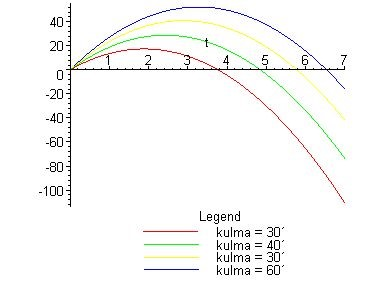
\includegraphics[width=\textwidth]{figures/bad-example.jpg}
\end{subfigure}
\begin{subfigure}{0.49\textwidth}
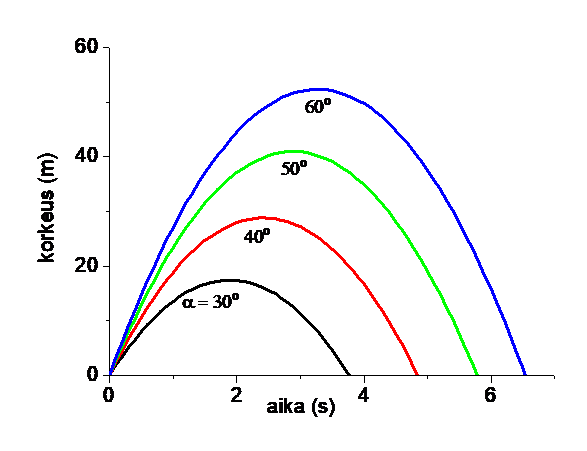
\includegraphics[width=\textwidth]{figures/good-example.png}
\end{subfigure}
\caption[This is a short caption.]{Diagrams should be edited before publication. The diagram on the right is an edited version of the one on the left.}
\label{fig:huolittelu}
\end{figure}

\begin{figure}
\centering
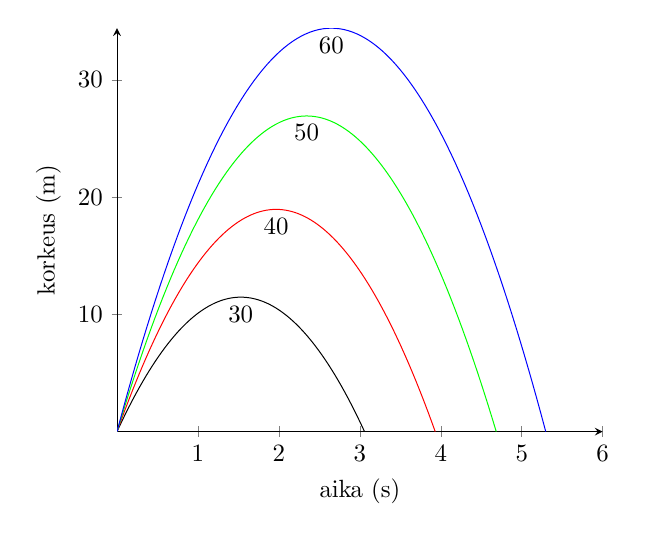
\begin{tikzpicture}[scale=0.9]
\begin{axis}[axis lines=center,
            xlabel={aika (s)},
            xlabel near ticks,
            ylabel={korkeus (m)},
            ylabel near ticks,
            xmin=0, xmax=6, ymin=0]
\addplot[color=black,
        domain=0:30*sin(30)/(0.5*9.81),
        samples=101]
        {30*sin(30)*x - 0.5*9.81*x^2}
        node[color=black, midway, below]{\ang{30}};
\addplot[color=red,
        domain=0:30*sin(40)/(0.5*9.81),
        samples=101]
        {30*sin(40)*x - 0.5*9.81*x^2}
        node[color=black, midway, below]{\ang{40}};
\addplot[color=green,
        domain=0:30*sin(50)/(0.5*9.81),
        samples=101]
        {30*sin(50)*x - 0.5*9.81*x^2}
        node[color=black, midway, below]{\ang{50}};
\addplot[color=blue,
        domain=0:30*sin(60)/(0.5*9.81),
        samples=101]
        {30*sin(60)*x - 0.5*9.81*x^2}
        node[color=black, midway, below]{\ang{60}};
\end{axis}
\end{tikzpicture}
\caption{An example of a graph along the lines of Figure \ref{fig:huolittelu} drawn using \texttt{pgfplots}.}
\label{fig:pgf-esimerkki}
\end{figure}

\section{Tables}

Taulukot sopivat hyvin erityisesti numeerisen informaation esittämiseen tiiviissä muodossa. Kuvien tapaan taulukot numeroidaan ja varustetaan otsikolla, kuten taulukossa. Taulukkoteksti sijoitetaan samalle sivulle taulukon kanssa ja taulukon yläpuolelle. Suureet, lyhenteet ja symbolit selitetään tarvittaessa tekstissä. Kaikkiin taulukoihin on viitattava tekstissä, mieluummin ennen taulukkoa. Taulukon keskeinen sanoma ja tulkintaohjeet selitetään tekstissä.

Taulukon sarakkeet otsikoidaan, ja suureet sekä yksiköt laitetaan näkyviin. Jos otsikkoriviä tarvitsee erottaa muusta taulukosta, tee se korostamalla (\verbcommand{emph}). Taulukon järjestyksellä on suuri merkitys. Jokaista solua ei pidä ympäröidä reunaviivalla, koska taulukosta tulee raskaslukuinen. Lisää vaakaviiva taulukon ylä- ja alareunaan. Vaakaviivoja voi käyttää esimerkiksi 4--5 rivin välein, ellei tietoja muuten ole jaettu kategorioihin tai selkeys sitä vaadi. Sarakkeen numeroarvot tasataan desimaalipilkun kohdalta, jolloin arvoja on helppo vertailla. Tämä tapahtuu \LaTeX{}issa helposti \texttt{siunitx}-paketin \parencite{siunitx} taulukkomateriaalin avulla. Tavoitteena on, että suureet ilmaistaan SI-yksikössä ja käytetään joko vakiintuneita etuliitteitä tai kymmenen potenssin muotoja siten, että ne voidaan laittaa otsikkoriville (katso tässäkin \texttt{siunitx}). Muutamia suosituksia taulukoiden ja kuvien käytöstä löydät lähteestä \parencite{pubadvice2009}.

Tables are convenient for presenting information in a concise way, especially numerical data. Tables have numbered captions, see Table \ref{tab:taulukkoesimerkki} for an example. The caption is placed on the same page but above the table, unlike the captions that accompany figures. You must refer to all the tables in the body text. In addition, you must discuss the content of any tables in the body text to ensure that readers understand their relevance.

Mark the titles of the columns and units clearly. You can use \verbcommand{emph} to highlight the titles, if necessary. The order of the columns and rows must be carefully considered. Do not surround all the cells with a border, as it may make your table harder to read. Put a line on top and bottom of the table. You can add a horizontal line between every 4–5 rows, if the data is not grouped into categories. The numbers are aligned at the decimal point for easy comparison. This is easily done in \LaTeX{} using the tabular material from the \texttt{siunitx} package \parencite{siunitx}. You should preferably use SI units, established prefixes and rewrite large numbers so that the power of ten should be placed in the title of the column instead of each row, if possible. More suggestions can be found in \parencite{pubadvice2009}.

\begin{table}
\centering
\caption{An example of evaporation conditions in two different thin film structures.}
\label{tab:taulukkoesimerkki}
% Making scarce use of table lines is recommended
% for clarity. Even the outer lines are generally
% not needed! Use the siunitx package provided
% S column type for easy decimal alignment.
\begin{tabular}{c|S[table-format=3.1] S[table-format=1.2] S[table-format=2.1e-1] S[table-format=2.1] S[table-format=2.0]@{--}S[table-format=3.0] S[table-format=1.1]}
    \hline
    compound & {thickness} & {correction} & {pressure} & {temperature} & \multicolumn{2}{c}{current} & {velocity} \\[-0.5ex]
    % The syntax \\[<length>] inserts a vertical
    % space of <length> in addition to the normal
    % new line action provided by \\. This should
    % apply in any situation.
    & {(\si{\nano\metre})} & & {(\si{\milli\bar})} & {(\si{\degreeCelsius})} & \multicolumn{2}{c}{(\si{\milli\ampere})} & {(\si{\nano\metre\per\second})} \\\hline
    \ce{SiO2} & 181.0 & 1.10 & 3.0e-5 & 90.6 & 20 & 23 & 0.2 \\
    \ce{TiO2} & 122.1 & 1.55 & 15.0e-5 & 91.1 & 93 & 100 & 0.1 \\\hline
\end{tabular}
\end{table}

\section{Mathematical notation and equations}

Numbers are generally written using numerals for the sake of clarity, for example ``6 stages'' rather than ``six stages'', which is nevertheless strongly preferred to ``a couple of stages''. You should also use a thousand separator, i.e. instead of 55700125 write \SI{55700125}{}. Never omit the leading zero in decimals. A comma is used as a decimal separator in the Finnish language and a period in the English language. These details are covered by this template and the \texttt{siunitx} package \parencite{siunitx}, if allowed to do so.

Like numbers, it is advisable to abbreviate units of measurement. There is a space between the number and the unit, but you must keep them on the same line. The space is somewhat shorter than a word space, see 1.0 \si{\micro\metre} and \SI{1.0}{\micro\metre} for comparison. It is better to compile a table or graph than include a great deal of numerical values in the body text. Use precise language and put numbers on a scale (small, fast, expensive).

Use generally known and well defined concepts and standard conventions and symbols for representing them. New concepts should be defined when they appear in the text for the first time. Upper case and lower case letters mean different things in symbols and units of measurement. Do not use the same symbol to mean different things.

Strings of mathematical symbols such as $\Theta(n^2)$ are typeset in \LaTeX{} using the math mode. Simple formulas may be displayed within the body of the text without numbering. As an example of a highlighted formula, the Newton’s Second Law of Motion can be written in the following way:
\begin{equation}\label{eq:newtonsecondlaw}
    m\mathbf{a} = \mathbf{F},
\end{equation}
where $m$ denotes the mass of an object, $\mathbf{a}$ its acceleration, and $\mathbf{F}$ the net force it experiences. Please note that all the variables must be defined at the point of their first appearance. The formulae are shown in a different typeface on purpose and the symbols are almost always italicised. Vectors can be written in boldface as above (the convention in printed material) or with an arrow, such as $\vec{v}$. Dimensional numbers can be written using the \verbcommand{SI} command:
\begin{equation*}
    \Vert\mathbf{F}\Vert = m\Vert\mathbf{a}\Vert = \SI{10}{\kilogram} \cdot \SI{9.81}{\metre\per\second\squared} = \SI{98.1}{\newton}.
\end{equation*}

Mathematical formulae are numbered, if they are written on separate lines and referred to in the main body of the text. The number is usually put in parenthesis and right aligned, see equation \eqref{eq:newtonsecondlaw} for an example. Include any punctuation (commas, periods) surrounding an equation in the equations themselves, such as shown in \eqref{eq:newtonsecondlaw}. Occasionally the elements of mathematical text are preceded by an identifier, such as Definition 1 or Theorem 1 \parencite{matohje2009}.

Do not start a sentence with a mathematical symbol but add some word, such as the name or type of the symbol in front of it. Variables, such as $x$ and $y$, are generally presented in italics, whereas elementary functions, special functions and operators are not: $\sin(2x + y)$ or
\begin{equation*}
    \lim_{x \rightarrow -1}\frac{x^2 - 1}{x + 1} = -2.
\end{equation*}
As a rule of thumb, it is best to rely on the automated formatting of an equation editor, such as the one provided by \LaTeX{} \parencite{notsoshort}.

Even those requiring different chemical symbols are not left without support by the \LaTeX{} system. Molecular formulae and stoichiometric equations, such as \ce{CH3CH2CH2COOH} and
\begin{center}
    \ce{N2 (g) + 3 H2 (g) <=> 2 NH3 (g)}
\end{center}
are typeset using the \texttt{mhchem} package \parencite{mhchem}, and complete structural formulae can be constructed with the aid of the \texttt{chemfig} package \parencite{chemfig}. The Lewis structure of tellurium tetrafluoride (\ce{TeF4}) is shown as an example of the latter.
\begin{center}
    \chemfig{\lewis{0:,Te}
    (-[:90]\lewis{0:2:4:,F})
    (-[:270]\lewis{0:4:6:,F})
    (<:[:135]\lewis{1:3:5:,F})
    (<[:225]\lewis{3:5:7:,F})
    }
\end{center}
There is a learning curve to writing these elements, especially the structural formulae, but it is good to know that there are ways of accomplishing them.

\section{Programs and algorithms}

Codes and algorithms are written using a \texttt{monospaced font}. If the length of the code or algorithm is less than 10 lines and you do not refer to it later on in the text, you can present it similarly to formulas. If the code is longer but shorter than a page, you present like a figure (see Program \ref{prog:esimerkki}) titled ``Program'' or ``Algorithm''. See the typesetting commands in this template for a method of setting the name manually.

You should add some comments to the code and indent it consistently. The actions performed by the code must be outlined in broad terms in the body text. Line numbers make it much easier to refer to the code in the text. \LaTeX{} includes a package called \texttt{listings} \parencite{listings,notsoshort}, which can handle code very conveniently, include real code files, add row numbers, and highlight the reserved words. Use this for any code representation in \LaTeX.

\renewcommand{\lstlistingname}{Program}
\lstinputlisting
    [float,
    caption={An example of presenting a program source code.},
    label=prog:esimerkki,
    language=C,
    numbers=left,
    morekeywords={CharPair}]
    {code/example-code.c}